\documentclass{article}
\usepackage{amsmath}
\usepackage{amssymb}
\usepackage{geometry}
\usepackage{tikz}
\usetikzlibrary{shapes,arrows,positioning}
\usepackage{booktabs}
\usepackage{graphicx}
\usepackage{subcaption}
\usepackage{multirow}

\begin{document}

\title{An Interpretable Statistical Surrogate of Activated Sludge Systems that Preserves Mass Conservation and Component Non-Negativity}

\maketitle

\section*{Nomenclature}
\begin{tabbing}
\hspace{2.5cm} \= \kill
$A$ \> Full-row-rank invariant matrix defining the null space of the stoichiometric matrix \\
$B$ \> Latent component-space parameter matrix of the unconstrained surrogate \\
$c_{in}$ \> Influent ASM component concentration vector ($c_{in} \in \mathbb{R}^{F}$) \\
$c_{out}$ \> True steady-state effluent ASM component concentration vector ($c_{out} \in \mathbb{R}^{F}$) \\
$c_{raw}$ \> Unconstrained surrogate prediction of the effluent ASM component state \\
$c^*$ \> Final non-negative, invariant-projected ASM component prediction \\
$c_{aff}$ \> Orthogonal affine projection of the raw prediction \\
$D$ \> Total dimension of the second-order feature map \\
$F$ \> Number of mechanistic ASM components \\
$I_{comp}$ \> Composition matrix mapping ASM components to measured composites ($I_{comp} \in \mathbb{R}^{K \times F}$) \\
$K$ \> Number of measured composite variables \\
$M$ \> Effective identifiable affine matrix in measured space ($M \in \mathbb{R}^{K \times D}$) \\
$M_{op}$ \> Number of operational variables \\
$P_{adm}$ \> Orthogonal projector onto the admissible change space \\
$P_{inv}$ \> Orthogonal projector onto the row space of $A$ \\
$R$ \> Number of reactions in the mechanistic model \\
$u$ \> Operational input vector ($u \in \mathbb{R}^{M_{op}}$) \\
$y$ \> True measured effluent composite vector ($y \in \mathbb{R}^{K}$) \\
$y^*$ \> Deployed projected measured prediction \\
$y_{raw}$ \> Unconstrained raw measured prediction \\
$\nu$ \> Stoichiometric matrix ($\nu \in \mathbb{R}^{R \times F}$) \\
$\xi$ \> Net reaction progress vector \\
$\phi$ \> Partitioned second-order feature map \\
$\otimes$ \> Kronecker product \\
\end{tabbing}

\section{Introduction}

Water pollution presents a critical environmental and public health challenge worldwide, with particularly severe repercussions in developing nations (Lin et al., 2022; Madhav et al., 2020). Biological wastewater treatment systems, particularly those based on the activated sludge process, are the dominant approach applied to combat this issue (Duan et al., 2022). However, their modeling and analysis present formidable engineering and computational challenges (Xiao et al., 2025). The underlying biophysical mechanisms are governed by the Activated Sludge Models (ASM) (Henze et al., 2006), which rely on coupled, multiplicative non-linear kinetic expressions to describe microbial growth and substrate consumption. This inherent non-linearity limits the practical application of transparent analytical methods for process design, frequently forcing engineers to rely on iterative trial-and-error approaches or computationally expensive heuristic algorithms (Aboagye et al., 2021; Padron-Paez et al., 2020).

In response to the computational and mathematical complexity inherent in non-linear Activated Sludge Models, research has increasingly focused on developing surrogate models to approximate the behavior of biological wastewater treatment systems (Bhosekar \& Ierapetritou, 2018; Durkin et al., 2024; Tsochatzidi et al., 2025). Traditional approaches have explored linearization techniques (Li et al., 2020; Yang et al., 2014) and multivariable polynomial fitting (Ahn et al., 2014; Kim et al., 2009; Lim et al., 2011). While linear methods like Partial Least Squares (PLS) offer interpretable mappings, they inherently struggle to capture the severe non-linearities of microbial kinetics without extensive feature engineering. To overcome these limitations, the machine learning (ML) paradigm has emerged as a powerful route for approximating highly non-linear wastewater-treatment behavior (Croll et al., 2023; Nazlabadi et al., 2021). A wide array of data-driven algorithms—ranging from distance-based methods like k-Nearest Neighbors (k-NN) and PLS (Khatri et al., 2020; Wold et al., 2001), to kernel methods like Support Vector Regression (SVR) (Fang et al., 2011), tree-based ensembles such as Random Forest (RF), AdaBoost, XGBoost, LightGBM, and CatBoost (Sadri Moghaddam \& Mesghali, 2023; Wang et al., 2025; Yang et al., 2025), and Artificial Neural Networks (ANN) (Asadi et al., 2017; Bagherzadeh et al., 2021; Mao et al., 2024)—have demonstrated strong predictive capabilities for effluent quality. 

Despite their predictive accuracy, these standard ML algorithms suffer from a fundamental structural blindness: they map operational inputs $u \in \mathbb{R}^{M_{op}}$ and influent conditions $c_{in}$ directly to measured outputs, minimizing empirical risk strictly in the observation space. In activated sludge systems, however, the true physical state is defined by a latent ASM component vector $c \in \mathbb{R}^F$, where $F$ is the number of mechanistic components (e.g., soluble substrate, autotrophic biomass, ammonium). The stoichiometric matrix $\nu \in \mathbb{R}^{R \times F}$ dictates how these components interact across $R$ reactions. This implies strict conservation laws of the form $Ac = Ac_{in}$, where $A \in \mathbb{R}^{q \times F}$ is a full-row-rank matrix whose transposed rows form a basis for $\operatorname{null}(\nu)$, such that $A\nu^T = 0$. Plant operators and simulators rarely observe $c$ directly; instead, they observe a measured composite vector $y \in \mathbb{R}^K$, defined by a linear composition map $y = I_{comp}c$, where $I_{comp} \in \mathbb{R}^{K \times F}$. 

By bypassing the latent component space $\mathbb{R}^F$, black-box regressors (such as PLS, k-NN, SVR, RF, AdaBoost, XGBoost, LightGBM, CatBoost, and ANN) can accurately fit observed effluent aggregates while implying a physically impossible redistribution of the underlying ASM components. To make this concrete, consider an ASM-flavored miniature system with three components: soluble substrate ($S_S$), particulate substrate ($X_S$), and ammonium ($S_{NH}$). Let a simplified reaction convert $S_S$ to $X_S$ without altering ammonium ($\nu = [-1, 1, 0]$). An admissible invariant basis preserving total COD equivalents and ammonium is $A = \left[\begin{smallmatrix} 1 & 1 & 0 \\ 0 & 0 & 1 \end{smallmatrix}\right]$. If the measured outputs are total COD and ammonium ($I_{comp} = A$), and the influent is $c_{in} = [10, 10, 5]^T$, a raw surrogate might predict an unphysical effluent state $c_{raw} = [-1, 21, 5]^T$. The measured output is $y_{raw} = I_{comp}c_{raw} = [20, 5]^T$. Crucially, the physically feasible state $c = [0, 20, 5]^T$ produces the exact same measured output $y = [20, 5]^T$. A measured-space-only correction cannot distinguish between these two states, allowing physically absurd internal states to masquerade as accurate predictions.

This study addresses this epistemological and physical mismatch through the development of Invariant-Constrained Second-Order Regression (ICSOR), a physics-informed surrogate framework for steady-state activated sludge systems. ICSOR is designed to answer a precise question: given a steady-state influent state and operating condition, what measured effluent state should be predicted if the underlying ASM component state must satisfy the stoichiometric invariants of the reaction network and remain componentwise non-negative? 

To achieve this, ICSOR employs a partitioned second-order feature map $\phi(u, c_{in})$ that explicitly separates operational variables (which alter the process environment) from influent concentrations (which dictate the material inventory). By retaining full vectorized quadratic blocks via the Kronecker product (e.g., $u \otimes u$, $c_{in} \otimes c_{in}$, and $u \otimes c_{in}$), the model transparently captures all pairwise non-linear operation-loading interactions. Specifically, these bilinear terms naturally approximate the multiplicative interactions inherent in the biological processes, such as the biomass-substrate coupling characteristic of Monod-type kinetics. Crucially, the raw surrogate prediction is corrected in the latent component space before being collapsed to measured outputs. This correction is executed in two stages: first, an orthogonal affine projection maps the raw prediction onto the invariant-consistent set ($Ac = Ac_{in}$); second, if this affine projection yields negative component concentrations, a strictly convex quadratic program (QP) finds the closest Euclidean point on the intersection of the invariant affine set and the non-negative orthant ($c \ge 0$). Component non-negativity guarantees composite non-negativity, provided the relevant rows of $I_{comp}$ are entrywise non-negative.

The objective of this article is to formulate the ICSOR framework as an analytically structured surrogate and to evaluate its efficacy on a standalone Continuous Stirred Tank Reactor (CSTR). By comparing ICSOR against the aforementioned unconstrained measured-space baselines, this study assesses whether the proposed model can achieve competitive predictive accuracy while explicitly guaranteeing the parsimony, interpretability, and rigorous physical consistency required for reliable process analysis. The framework presented herein is strictly bounded to steady-state predictions; while it guarantees stoichiometric invariance and non-negativity, it does not claim to enforce full kinetic or thermodynamic feasibility, nor does it replace dynamic trajectory simulators. Instead, it occupies a necessary middle ground: a surrogate simple enough to have its affine core estimated from data by least squares, yet mathematically constrained to respect the fundamental mass balances of wastewater engineering.

\section{Theory and Calculation}

The mathematical framework of Invariant-Constrained Second-Order Regression (ICSOR) is developed to reconcile the predictive flexibility of data-driven surrogates with the strict conservation laws of mechanistic modeling. The framework operates across two linked spaces: the latent ASM component space, where stoichiometry and non-negativity are physically defined, and the measured composite space, where prediction targets are observed and evaluated.

\subsection{Physical Scope, State Spaces, and Notation}

A fixed reactor block or process unit represented by quasi-steady samples is considered. The system boundary is identical to the boundary used to define the influent and effluent state vectors. Any external source or sink crossing that boundary must be explicitly represented in the adopted stoichiometric model; otherwise, it is excluded from the claim of invariant preservation. 

Let $M_{op}$ be the number of operational variables, $F$ the number of ASM components, $K$ the number of measured composite variables, and $R$ the number of reactions. Single-sample vectors are written as column vectors. The following state spaces and operators are defined:
\begin{itemize}
    \item $u \in \mathbb{R}^{M_{op}}$: Operational input vector (e.g., hydraulic retention time, aeration intensity).
    \item $c_{in} \in \mathbb{R}^{F}$: Influent ASM component concentration vector.
    \item $c_{out} \in \mathbb{R}^{F}$: True steady-state effluent ASM component concentration vector.
    \item $c_{raw} \in \mathbb{R}^{F}$: Unconstrained surrogate prediction of the effluent ASM component state.
    \item $c^* \in \mathbb{R}^{F}$: Final non-negative, invariant-projected ASM component prediction.
    \item $y \in \mathbb{R}^{K}$: Measured effluent composite vector.
    \item $I_{comp} \in \mathbb{R}^{K \times F}$: Composition matrix mapping ASM component concentrations to measured composite variables, such that $y = I_{comp}c_{out}$.
    \item $\nu \in \mathbb{R}^{R \times F}$: Stoichiometric matrix.
\end{itemize}

The linear composition map $I_{comp}$ is standard in wastewater modeling. In the common case where composites (e.g., total COD, total nitrogen, TSS) are formed by summing relevant component concentrations with non-negative conversion factors, the rows of $I_{comp}$ are entrywise non-negative. This sign structure is critical: non-negative component predictions ($c^* \ge 0$) mathematically imply non-negative measured composites ($y^* \ge 0$) only under this specific condition.

\subsection{Stoichiometric Structure and Conserved Quantities}

Let $\nu \in \mathbb{R}^{R \times F}$ be the stoichiometric matrix written in the adopted ASM component basis. For a steady-state sample, define the net reaction progress vector $\xi \in \mathbb{R}^{R}$, scaled into concentration-equivalent units, such that the net change across the control volume is:
\begin{equation}
c_{out} - c_{in} = \nu^T \xi
\end{equation}
The vector $\xi$ is rarely observed. To eliminate it and isolate the conserved quantities, a full-row-rank matrix $A \in \mathbb{R}^{q \times F}$ is introduced, whose transposed rows form a basis of $\operatorname{null}(\nu)$. Equivalently, $A \nu^T = 0$. Multiplying the stoichiometric change relation by $A$ yields:
\begin{equation}
A(c_{out} - c_{in}) = A \nu^T \xi = 0 \quad \implies \quad A c_{out} = A c_{in}
\end{equation}
Each row of $A$ represents one independent conserved combination of ASM components (e.g., COD equivalents or nitrogen balances) implied by the reaction network. The invariant relation $A c_{out} = A c_{in}$ forms the affine physical constraint that any credible surrogate must satisfy.

To make this concrete, consider a miniature 2-component system where soluble substrate ($c_1$) is converted to particulate substrate ($c_2$) without net loss: $\nu = [-1, 1]$. The null space is spanned by $A = [1, 1]$. The invariant relation becomes $c_{out,1} + c_{out,2} = c_{in,1} + c_{in,2}$. The reaction may redistribute material, but it cannot alter the conserved total.

\subsection{Unconstrained Surrogate in ASM Component Space}

In activated sludge systems, operational variables ($u$) alter the process environment, while influent concentrations ($c_{in}$) dictate the material inventory. Treating them as interchangeable inputs obscures their physical roles. ICSOR partitions these inputs using an engineered second-order feature map:
\begin{equation}
\phi(u, c_{in}) = \begin{bmatrix}
1 \\
u \\
c_{in} \\
u \otimes u \\
c_{in} \otimes c_{in} \\
u \otimes c_{in}
\end{bmatrix} \in \mathbb{R}^{D}
\end{equation}
where $\otimes$ denotes the Kronecker product under column-wise vectorization, yielding a feature dimension $D = 1 + M_{op} + F + M_{op}^2 + F^2 + M_{op}F$. 

The unconstrained raw surrogate is defined in the latent component space as $c_{raw} = B \phi(u, c_{in})$, where $B \in \mathbb{R}^{F \times D}$. To ground this mathematically and physically, $B$ is partitioned conformably with the feature map:
\begin{equation}
c_{raw} = b + W_u u + W_{in} c_{in} + \Theta_{uu}(u \otimes u) + \Theta_{cc}(c_{in} \otimes c_{in}) + \Theta_{uc}(u \otimes c_{in})
\end{equation}
with parameter blocks defined as $W_u \in \mathbb{R}^{F \times M_{op}}$, $W_{in} \in \mathbb{R}^{F \times F}$, $b \in \mathbb{R}^{F}$, $\Theta_{uu} \in \mathbb{R}^{F \times M_{op}^2}$, $\Theta_{cc} \in \mathbb{R}^{F \times F^2}$, and $\Theta_{uc} \in \mathbb{R}^{F \times (M_{op}F)}$. 

Each block has a distinct engineering interpretation in the latent space: $W_u u$ captures first-order operating effects; $W_{in} c_{in}$ captures direct carry-through of influent composition; $\Theta_{uu}$ and $\Theta_{cc}$ capture self-quadratic non-linearities; and crucially, $\Theta_{uc}(u \otimes c_{in})$ captures the operation-loading interactions that drive biological kinetics. However, because $c_{raw}$ is purely data-driven, it is not guaranteed to satisfy the invariant relation $A c_{raw} = A c_{in}$, nor is it guaranteed to be non-negative.

\subsection{Projection onto the Invariant-Consistent Non-Negative Set}

To enforce physical discipline, the raw prediction must be corrected. The invariant-consistent non-negative feasible set for a given influent state is defined as:
\begin{equation}
\mathcal{S}_+(c_{in}) = \{ c \in \mathbb{R}^{F} : A c = A c_{in}, \; c \ge 0 \}
\end{equation}
ICSOR corrects the raw surrogate by finding the closest Euclidean point in this feasible set. This is formulated as a strictly convex quadratic program (QP):
\begin{equation}
c^* = \arg\min_{c \in \mathbb{R}^{F}} \; \frac{1}{2} \lVert c - c_{raw} \rVert_2^2 \quad \text{subject to} \quad A c = A c_{in}, \quad c \ge 0
\end{equation}
Because the objective is strictly convex and the feasible set is closed and non-empty (assuming $c_{in} \ge 0$), the minimizer $c^*$ exists and is unique. Because this metric is Euclidean in raw concentration coordinates, component scaling directly influences the magnitude and direction of the correction.

This formulation contains the orthogonal affine projection as a reference solution. If the non-negativity constraint is dropped, the closed-form affine projection is:
\begin{equation}
c_{aff} = P_{adm} c_{raw} + P_{inv} c_{in}
\end{equation}
where $P_{inv} = A^T(A A^T)^{-1} A$ is the orthogonal projector onto the row space of $A$, and $P_{adm} = I_F - P_{inv}$ is the projector onto the admissible change space. 

In computational deployment, solving the full $F$-dimensional QP is unnecessary. Let $N_A \in \mathbb{R}^{F \times (F-q)}$ be a matrix whose orthonormal columns span $\operatorname{null}(A)$. Every point in the affine set can be parameterized as $c = c_{aff} + N_A z$ for some reduced coordinate vector $z \in \mathbb{R}^{F-q}$. Because $N_A$ has orthonormal columns, the Euclidean metric is preserved ($z^T N_A^T N_A z = z^T z$), and the correction reduces to:
\begin{equation}
\min_{z \in \mathbb{R}^{F-q}} \; \frac{1}{2} z^T z \quad \text{subject to} \quad N_A z \ge -c_{aff}
\end{equation}
The correction is evaluated hierarchically: if $c_{raw}$ is feasible, it is retained; if only invariants are violated, $c_{aff}$ is used; the reduced QP is solved only when $c_{aff}$ contains negative components.

\subsection{Collapse to Measured Output Space and Blockwise Interpretability}

Practical prediction targets are measured composites, not latent components. The final deployed prediction is obtained by collapsing the corrected component state:
\begin{equation}
y^* = I_{comp} c^*
\end{equation}
Crucially, the correction must occur \textit{before} the collapse. A measured-space-only correction cannot distinguish between physically distinct component states that happen to yield the same composite aggregates.

Before positivity constraints activate, the measured prediction induced by the affine projector is $y_{aff} = I_{comp} c_{aff}$. Substituting the definition of $c_{aff}$ yields the affine measured-space core:
\begin{equation}
y_{aff} = G B \phi(u, c_{in}) + H c_{in}
\end{equation}
where $G = I_{comp} P_{adm}$ and $H = I_{comp} P_{inv}$. Defining the effective identifiable affine matrix as $M = G B \in \mathbb{R}^{K \times D}$, the model becomes:
\begin{equation}
y_{aff} = M \phi(u, c_{in}) + H c_{in}
\end{equation}

While the latent component-space matrix $B$ is not uniquely identifiable from measured data, the effective affine core $M$ is. To provide direct engineering interpretability, $M$ can be partitioned conformably with the feature map into effective measured-space blocks:
\begin{equation}
M = \begin{bmatrix}
b_y & W_{u,y} & W_{in,y} & \Theta_{uu,y} & \Theta_{cc,y} & \Theta_{uc,y}
\end{bmatrix}
\end{equation}
where $b_y = G b$, $W_{u,y} = G W_u$, $W_{in,y} = G W_{in}$, $\Theta_{uu,y} = G \Theta_{uu}$, $\Theta_{cc,y} = G \Theta_{cc}$, and $\Theta_{uc,y} = G \Theta_{uc}$. Substituting these blocks into the affine-core model and collecting the first-order influent terms yields:
\begin{equation}
y_{aff} = b_y + W_{u,y} u + (W_{in,y} + H)c_{in} + \Theta_{uu,y}(u \otimes u) + \Theta_{cc,y}(c_{in} \otimes c_{in}) + \Theta_{uc,y}(u \otimes c_{in})
\end{equation}
This blockwise expression is the cornerstone of the model's interpretability. A process engineer can directly inspect $W_{u,y}$ to understand the effective linear sensitivity of measured composites (e.g., effluent total nitrogen) to operational changes (e.g., aeration intensity). Similarly, $\Theta_{uc,y}$ explicitly quantifies how shifts in influent loading modify those operational sensitivities in the measured space. 

\subsection{Estimation and Epistemological Boundaries}

This affine relation dictates the epistemology of the framework. For a dataset of $N$ steady-state samples, let $\Phi \in \mathbb{R}^{N \times D}$ be the feature matrix, $Y \in \mathbb{R}^{N \times K}$ the measured output matrix, and $C_{in} \in \mathbb{R}^{N \times F}$ the influent state matrix. Defining the transformed target $\widetilde{Y} = Y - C_{in} H^T$, the dataset-level estimation equation is:
\begin{equation}
\widetilde{Y} = \Phi M^T + E
\end{equation}
Measured composite data uniquely identify the affine core $M$ via the least-squares pseudoinverse estimator $\widehat{M}^T = \Phi^+ \widetilde{Y}$. However, they do \textit{not} uniquely identify the latent component-space matrix $B$. If $N_B \in \mathbb{R}^{F \times D}$ satisfies $G N_B = 0$, then $G(B + N_B) = M$. 

Consequently, the final deployed predictor is decomposed as:
\begin{equation}
y^* = y_{aff} + \delta_+(u, c_{in})
\end{equation}
where $\delta_+(u, c_{in}) = I_{comp}(c^* - c_{aff})$ is the sample-specific positivity correction. The data identify the globally affine core $y_{aff}$ (and its interpretable blocks), while the non-linear correction $\delta_+$ relies on fixing a chosen latent representative for $B$. If the minimum-Frobenius-norm exact representative $\widehat{B}_{ls} = G^+ \widehat{M}$ is chosen, it induces a compatible affine core $\widehat{M}_G = G G^+ \widehat{M}$. This compatible core equals the unconstrained least-squares fit $\widehat{M}$ only when $\widehat{M}$ already lies perfectly in $\operatorname{range}(G)$. This delineates exactly what the surrogate learns from data versus what it enforces through physical geometry.

\section{Methodology}

This section documents the computational protocol used to evaluate the proposed Invariant-Constrained Second-Order Regression (ICSOR) model against a suite of classical regressors. The comparison was designed to isolate the effect of model structure and physical constraint handling: every model was exposed to the same synthetic operating scenarios, the same measured effluent targets, and the same row-wise train-test partitions. Because the classical regressors predict directly in measured-output space and do not produce a latent component-space estimate $c_{raw}$, no post-hoc constraint projection was applied to their outputs. Thus, the cross-model comparison ranks all models on their deployed measured-output predictions, while the physical diagnostics available exclusively from ICSOR are reported separately.

\subsection{Mechanistic Dataset and Simulation Domain}

All benchmark data were generated from a standalone steady-state continuous stirred tank reactor (CSTR) simulator based on the Activated Sludge Model No.\ 2d with two-step nitrification (ASM2d-TSN). The mechanistic description contained $R = 28$ biological and chemical processes acting on $F = 21$ ASM state variables, and a linear composition map $I_{comp} \in \mathbb{R}^{K \times F}$ with $K = 6$ from the latent state space to six measured effluent composites: chemical oxygen demand (COD), total nitrogen (TN), total Kjeldahl nitrogen (TKN), total phosphorus (TP), total suspended solids (TSS), and volatile suspended solids (VSS).

The simulation domain was sampled using Latin hypercube sampling (LHS) to ensure uniform coverage of the joint input space. A total of 10,000 valid steady-state samples were generated with random seed 42. Each sample was defined by $M_{op} = 2$ operating variables and $F = 21$ influent state variables. The operating variables were the hydraulic retention time and aeration level, sampled as $\mathrm{HRT} \in [6,36]$~h and $\mathrm{Aeration} \in [0.5,2.5]$. The influent-state sampling ranges are presented in Table~\ref{tab:influent_ranges}.

\begin{table}[htbp]
\centering
\caption{Influent ASM2d-TSN state variable sampling ranges. All concentrations are expressed in the native ASM2d units: g~COD/m\textsuperscript{3} for organic and biomass fractions, g~N/m\textsuperscript{3} for nitrogen species, g~P/m\textsuperscript{3} for phosphorus species, mol/m\textsuperscript{3} for alkalinity, g~O\textsubscript{2}/m\textsuperscript{3} for dissolved oxygen, and g~TSS/m\textsuperscript{3} for solids fractions.}
\label{tab:influent_ranges}
\begin{tabular}{@{}llcc@{}}
\toprule
\textbf{Category} & \textbf{State Variable} & \textbf{Lower Bound} & \textbf{Upper Bound} \\
\midrule
\multirow{10}{*}{Dissolved}
 & $S_A$ (Soluble acetate) & 5 & 80 \\
 & $S_F$ (Soluble fermentable substrate) & 20 & 180 \\
 & $S_I$ (Soluble inert) & 10 & 90 \\
 & $S_{N2}$ (Dissolved nitrogen gas) & 0 & 2 \\
 & $S_{NH4}$ (Ammonium) & 12 & 55 \\
 & $S_{NO2}$ (Nitrite) & 0 & 3 \\
 & $S_{NO3}$ (Nitrate) & 0 & 8 \\
 & $S_{PO4}$ (Phosphate) & 2 & 18 \\
 & $S_{ALK}$ (Alkalinity) & 80 & 260 \\
 & $S_{O2}$ (Dissolved oxygen) & 0 & 0.5 \\
\midrule
\multirow{11}{*}{Particulate}
 & $X_I$ (Particulate inert) & 20 & 120 \\
 & $X_S$ (Particulate substrate) & 60 & 280 \\
 & $X_H$ (Heterotrophic biomass) & 15 & 100 \\
 & $X_{PAO}$ (Phosphate-accumulating organisms) & 5 & 60 \\
 & $X_{PP}$ (Polyphosphate) & 2 & 20 \\
 & $X_{PHA}$ (Polyhydroxyalkanoates) & 1 & 30 \\
 & $X_{AOB}$ (Ammonia-oxidizing bacteria) & 0.5 & 8 \\
 & $X_{NOB}$ (Nitrite-oxidizing bacteria) & 0.5 & 8 \\
 & $X_{TSS}$ (Total suspended solids) & 0 & 0 \\
 & $X_{MeOH}$ (Metal hydroxide) & 0 & 12 \\
 & $X_{MeP}$ (Metal phosphate) & 0 & 12 \\
\bottomrule
\end{tabular}
\end{table}

For each sampled influent-operating point, the effluent steady state was obtained by solving the nonlinear ASM2d-TSN algebraic balance equations under bound constraints. Although LHS independently samples the input space, the nonlinear ASM algebraic solver inherently acts as a physical filter: operating points leading to severe washout or non-viable states that fail to converge to a stable steady state within the prescribed residual tolerances are rejected. The generative procedure explicitly continued drawing new samples until exactly 10,000 valid, biologically viable steady-state points were collected. The primary solve used bound-constrained nonlinear least squares with lower and upper state bounds of $10^{-8}$ and 1500, variable, residual, and gradient tolerances of $10^{-9}$, and a maximum of 1200 function evaluations. Two starting points were tested for each sample: an initial guess assembled from the current influent state and the previous accepted solution, and a multistart perturbation of that initial guess. If neither trial reduced the maximum absolute residual below the configured acceptance threshold of 5.0, a dynamic-relaxation step was performed by integrating the governing residual dynamics for 20 days with a Backward Differentiation Formula (BDF) solver before re-solving the steady-state problem. Only solutions that both converged and satisfied the acceptance threshold were retained.

The accepted effluent ASM state $c_{out} \in \mathbb{R}^F$ was then collapsed through the composition matrix $I_{comp}$ to the six measured outputs $y = I_{comp} c_{out}$. The persisted dataset therefore contained operating variables $u$, influent component states $c_{in}$, influent measured composites $I_{comp} c_{in}$, effluent component states $c_{out}$, and effluent measured composites $y$. However, only the measured effluent composites were used as prediction targets in the cross-model benchmark.

\subsection{Construction of the Benchmark Dataset and Constraint Operators}

The stoichiometric matrix $\nu \in \mathbb{R}^{R \times F}$, corresponding to the Petersen matrix of the ASM2d-TSN reaction network, and the composition matrix $I_{comp} \in \mathbb{R}^{K \times F}$ were taken from the canonical ASM2d-TSN reference formulation used by the simulator. From the stoichiometric matrix, the component-space invariant matrix $A \in \mathbb{R}^{q \times F}$ was obtained as a basis of the left null space of $\nu$, consistent with the conservation law $A\nu^T = 0$ developed in Section~2. Concretely, the left null space of $\nu$ is equivalent to the right null space of $\nu^T$. This null space was computed using the \texttt{scipy.linalg.null\_space} function from SciPy (Virtanen et al., 2020), which internally performs a Singular Value Decomposition (SVD) and extracts the right singular vectors whose corresponding singular values fall below a numerically determined tolerance. The SVD-based approach was selected because it is numerically stable for rank-deficient matrices and yields an orthonormal basis, avoiding the ill-conditioning that can arise from direct factorization methods such as Gaussian elimination on the transpose. The resulting orthonormal column vectors were transposed to form the rows of $A$. To further stabilize the representation for downstream arithmetic, the entries of $A$ were rounded to five decimal places, entries with magnitude below $10^{-10}$ were set to zero, and each row was normalized by its first non-zero coefficient so that the leading non-trivial entry of every conserved-quantity row is unity.

A single supervised-learning dataset was assembled for the entire benchmark. Its features consisted of 23 physical inputs for every sample: the two operating variables $u \in \mathbb{R}^{M_{op}}$ and the 21 influent ASM state variables $c_{in} \in \mathbb{R}^{F}$. Its targets were the six measured effluent composites $y \in \mathbb{R}^{K}$. For ICSOR, the 21-component influent state vector $c_{in}$ additionally served as the constraint reference, so that the invariant projection and non-negativity correction could be enforced in the latent component space before collapse to measured outputs via $I_{comp}$.

Because the classical regressors predict directly in the measured-output space $\mathbb{R}^K$ and never construct a latent component prediction $c_{raw} \in \mathbb{R}^F$, no invariant or non-negativity projection was applied to their outputs. The raw measured-space prediction of each classical model constitutes its deployed prediction. By contrast, ICSOR's deployed prediction is the physically corrected output $y^* = I_{comp} c^*$ obtained after the invariant and non-negativity projection described in Section~2. All models shared exactly the same 23-feature input basis and the same six-target output basis, ensuring that any differences in predictive accuracy are attributable solely to model structure.

\subsection{Preprocessing and Split Management}

One common row-wise train-test split was created using a test fraction of 0.2 and random seed 42. On the 10,000-sample dataset, this yielded 8,000 training rows and 2,000 testing rows. All one-shot benchmark results reported in this study were produced from this common split so that differences in prediction accuracy could not be attributed to different train-test partitions.

The classical regressors were standardized by z-score normalization fitted on the training split only, separately for the feature matrix and the six-target output matrix. The fitted transforms were then applied to both training and test data, and all predictions were inverse-transformed back to the original measured units before metric evaluation. ICSOR was not standardized: feature scaling and target scaling were both disabled so that the influent component states remained in physical coordinates and the composition map $I_{comp}$ remained consistent with the formulation in Section~2.

\subsection{Hyperparameter Optimization}

The hyperparameters of all classical benchmark regressors were selected via Bayesian optimization using the Optuna framework. For each classical model, 50\% of the authoritative training pool was sampled, yielding a 4,000-row tuning subset. That subset was partitioned again with a 20\% validation fraction, producing 3,200 tuning-train rows and 800 tuning-validation rows. Each Optuna study used 100 trials, no wall-clock timeout, random seed 42, and validation mean squared error (MSE) as the objective function. The optimized hyperparameters selected by this procedure are reported in Table~\ref{tab:optuna_hyperparameters}.

\begin{table}[htbp]
\centering
\caption{Optuna-optimized hyperparameters for the classical benchmark regressors. ICSOR has no tunable hyperparameters beyond its analytical formulation.}
\label{tab:optuna_hyperparameters}
\small
\begin{tabular}{@{}lll@{}}
\toprule
\textbf{Model} & \textbf{Parameter} & \textbf{Selected Value} \\
\midrule
\multirow{5}{*}{XGBoost}
 & Number of trees & 250 \\
 & Learning rate & 0.03 \\
 & Maximum depth & 8 \\
 & Subsample fraction & 0.85 \\
 & Column subsample fraction & 0.80 \\
\midrule
\multirow{6}{*}{LightGBM}
 & Number of trees & 300 \\
 & Learning rate & 0.04 \\
 & Number of leaves & 45 \\
 & Minimum child samples & 8 \\
 & Subsample fraction & 0.85 \\
 & Column subsample fraction & 0.90 \\
\midrule
\multirow{5}{*}{CatBoost}
 & Iterations & 300 \\
 & Learning rate & 0.04 \\
 & Depth & 7 \\
 & Bagging temperature & 0.8 \\
 & Random strength & 0.5 \\
\midrule
\multirow{3}{*}{AdaBoost}
 & Number of estimators & 200 \\
 & Learning rate & 0.03 \\
 & Loss function & linear \\
\midrule
\multirow{2}{*}{Random Forest}
 & Number of trees & 400 \\
 & Bootstrap & true \\
\midrule
\multirow{3}{*}{SVR}
 & Kernel & RBF \\
 & Regularization $C$ & 15.0 \\
 & Epsilon $\epsilon$ & 0.03 \\
\midrule
\multirow{2}{*}{$k$-NN}
 & Number of neighbors $k$ & 7 \\
 & Weighting & distance \\
\midrule
\multirow{1}{*}{PLS}
 & Number of components & 6 \\
\midrule
\multirow{5}{*}{ANN (all depths)}
 & Activation & ReLU \\
 & Optimizer & Adam \\
 & L2 regularization $\alpha$ & $10^{-4}$ \\
 & Batch size & 64 \\
 & Maximum iterations & 500 \\
\midrule
ANN Shallow & Hidden layers & $(64)$ \\
ANN Medium & Hidden layers & $(96, 48)$ \\
ANN Deep & Hidden layers & $(128, 64, 32)$ \\
\bottomrule
\end{tabular}
\end{table}

Random seed 42 was used wherever the model family exposed stochastic initialization. ICSOR requires no hyperparameter tuning: its identifiable affine core $M$ is estimated in closed form by multivariate least squares, and the physical projection parameters are derived directly from the stoichiometric matrix $\nu$ and the composition matrix $I_{comp}$.

\subsection{Benchmark Models}

\subsubsection{ICSOR}

The ICSOR model was constructed exactly as described in Section~2. The input was partitioned into the operational vector $u \in \mathbb{R}^{M_{op}}$ ($M_{op} = 2$) and the influent component vector $c_{in} \in \mathbb{R}^{F}$ ($F = 21$). These were mapped through the partitioned second-order feature map defined in Eq.~(3):
\begin{equation*}
\phi(u, c_{in}) = \begin{bmatrix} 1, & u^T, & c_{in}^T, & (u \otimes u)^T, & (c_{in} \otimes c_{in})^T, & (u \otimes c_{in})^T \end{bmatrix}^T \in \mathbb{R}^D
\end{equation*}
yielding a total feature dimension of $D = 1 + 2 + 21 + 4 + 441 + 42 = 511$, comprising 1 bias term, 2 linear operational terms, 21 linear influent terms, 4 operational self-product terms, 441 influent self-product terms, and 42 operation-influent interaction terms. The identifiable affine core $\widehat{M} \in \mathbb{R}^{K \times D}$ was estimated by the multivariate least-squares pseudoinverse $\widehat{M}^T = \Phi^+ \widetilde{Y}$ as described in Section~2.6. A minimum-Frobenius-norm representative $\widehat{B}_{ls} = G^+ \widehat{M}$ was then fixed to enable latent-component-space prediction.

Raw component-space predictions $c_{raw} = \widehat{B}_{ls}\, \phi(u, c_{in})$ were corrected in two stages following the hierarchical procedure of Section~2.4: first, the orthogonal affine projection $c_{aff} = P_{adm}\, c_{raw} + P_{inv}\, c_{in}$ enforced the invariant relation $Ac = Ac_{in}$; second, when $c_{aff}$ contained negative components, the reduced-dimension quadratic program (Eq.~8) was solved using the Operator Splitting Quadratic Program (OSQP) solver with absolute and relative tolerances of $10^{-8}$, a maximum of 10,000 iterations, and enabled polishing and warm starts. The corrected component state $c^*$ was then collapsed to the measured output via $y^* = I_{comp}\, c^*$.

\subsubsection{Classical Regressors}

The classical benchmark contained eleven regressors, all trained on the same 23-input basis and all targeting the same six measured outputs: XGBoost, LightGBM, CatBoost, AdaBoost, Random Forest, Support Vector Regression (SVR), $k$-Nearest Neighbors ($k$-NN), Partial Least Squares (PLS), and three multilayer perceptrons (MLP) denoted shallow, medium, and deep. The Optuna-optimized hyperparameters for each model are listed in Table~\ref{tab:optuna_hyperparameters}.

The three MLP architectures are illustrated in Fig.~\ref{fig:mlp_architectures}. All three used the Rectified Linear Unit (ReLU) activation function, the Adam optimizer, L2 regularization coefficient $\alpha = 10^{-4}$, batch size 64, and a maximum of 500 training iterations with convergence tolerance $10^{-4}$.

\begin{figure}[htbp]
\centering
\begin{subfigure}[b]{0.32\textwidth}
\centering
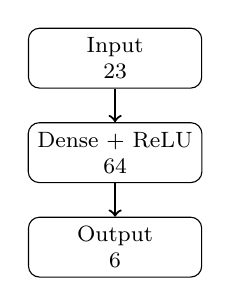
\begin{tikzpicture}[
    node distance=1.2cm,
    every node/.style={draw, rounded corners, minimum width=2.2cm, minimum height=0.7cm, align=center, font=\footnotesize},
    arrow/.style={->, thick}
]
\node (input) {Input\\23};
\node (h1) [below of=input] {Dense + ReLU\\64};
\node (output) [below of=h1] {Output\\6};
\draw[arrow] (input) -- (h1);
\draw[arrow] (h1) -- (output);
\end{tikzpicture}
\caption{Shallow $(64)$}
\end{subfigure}
\hfill
\begin{subfigure}[b]{0.32\textwidth}
\centering
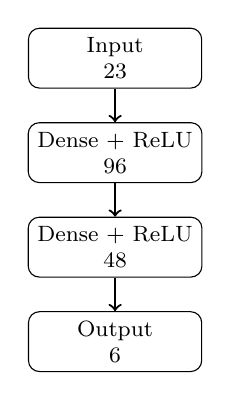
\begin{tikzpicture}[
    node distance=1.2cm,
    every node/.style={draw, rounded corners, minimum width=2.2cm, minimum height=0.7cm, align=center, font=\footnotesize},
    arrow/.style={->, thick}
]
\node (input) {Input\\23};
\node (h1) [below of=input] {Dense + ReLU\\96};
\node (h2) [below of=h1] {Dense + ReLU\\48};
\node (output) [below of=h2] {Output\\6};
\draw[arrow] (input) -- (h1);
\draw[arrow] (h1) -- (h2);
\draw[arrow] (h2) -- (output);
\end{tikzpicture}
\caption{Medium $(96, 48)$}
\end{subfigure}
\hfill
\begin{subfigure}[b]{0.32\textwidth}
\centering
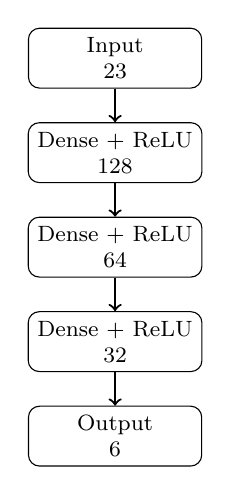
\begin{tikzpicture}[
    node distance=1.2cm,
    every node/.style={draw, rounded corners, minimum width=2.2cm, minimum height=0.7cm, align=center, font=\footnotesize},
    arrow/.style={->, thick}
]
\node (input) {Input\\23};
\node (h1) [below of=input] {Dense + ReLU\\128};
\node (h2) [below of=h1] {Dense + ReLU\\64};
\node (h3) [below of=h2] {Dense + ReLU\\32};
\node (output) [below of=h3] {Output\\6};
\draw[arrow] (input) -- (h1);
\draw[arrow] (h1) -- (h2);
\draw[arrow] (h2) -- (h3);
\draw[arrow] (h3) -- (output);
\end{tikzpicture}
\caption{Deep $(128, 64, 32)$}
\end{subfigure}
\caption{Multilayer perceptron architectures used in the classical benchmark. Each box denotes a fully connected layer followed by the specified activation function. The numbers indicate the layer width (number of neurons). All three architectures map 23 inputs to 6 measured outputs.}
\label{fig:mlp_architectures}
\end{figure}

The classical regressors produced predictions directly in the measured-output space $\mathbb{R}^K$. Because these models never construct a latent component-space prediction $c_{raw} \in \mathbb{R}^F$, there is no physically meaningful basis on which to apply the invariant or non-negativity projection developed in Section~2. Consequently, the raw measured-space output of each classical model constitutes its final deployed prediction and is used directly for metric evaluation.

\subsection{Prediction Taxonomy and Metric Definitions}

Before presenting the evaluation protocol, it is necessary to define precisely how the different types of predictions and their associated metrics are distinguished throughout this study.

\subsubsection{Raw and Projected Predictions}

For ICSOR, the term \textit{raw prediction} denotes the measured-space output obtained by collapsing the unconstrained component-space estimate without any physical correction, i.e., $y_{raw} = I_{comp}\, c_{raw}$. This prediction does not satisfy the stoichiometric invariants $Ac = Ac_{in}$ and may imply negative component concentrations. The term \textit{projected prediction} denotes the physically corrected measured-space output $y^* = I_{comp}\, c^*$, obtained after the invariant affine projection and, when necessary, the non-negativity quadratic program have been applied to $c_{raw}$ in the latent component space. The projected prediction is the deployed output of the ICSOR framework.

For the classical regressors, only raw predictions exist. Because these models map inputs directly to measured composites without ever constructing a latent component-space estimate, neither invariant projection nor non-negativity correction can be applied. The raw measured-space output is therefore also the deployed output.

\subsubsection{Effective Metrics}

To enable a fair cross-model comparison, the term \textit{effective prediction} is defined as the deployed output of each model: the projected prediction $y^*$ for ICSOR and the raw measured-space prediction $\hat{y}$ for each classical regressor. All cross-model rankings in this study are based exclusively on effective predictions. Correspondingly, the \textit{effective test metric} for a given performance measure (e.g., effective test RMSE) denotes that measure evaluated on the test set using each model's effective prediction, and the \textit{effective training metric} denotes the same measure evaluated on the training set.

\subsubsection{Regression Metrics}

Five standard regression metrics were employed throughout the evaluation, each computed as an aggregate over all $K = 6$ measured output targets. Let $y_i \in \mathbb{R}^K$ and $\hat{y}_i \in \mathbb{R}^K$ denote the observed and predicted measured vectors for sample $i$, respectively, over $N$ evaluation samples with $N_t = N \times K$ total scalar predictions. The metrics are:

\begin{enumerate}
\item \textbf{Coefficient of determination} ($R^2$): Defined as $R^2 = 1 - \sum_{j=1}^{K} \sum_{i=1}^{N} (y_{ij} - \hat{y}_{ij})^2 \Big/ \sum_{j=1}^{K} \sum_{i=1}^{N} (y_{ij} - \bar{y}_j)^2$, where $\bar{y}_j$ is the mean of target $j$ over the evaluation set. Individual per-target $R^2$ scores are averaged uniformly across the $K$ targets.

\item \textbf{Mean squared error} (MSE): $\mathrm{MSE} = \frac{1}{N_t} \sum_{j=1}^{K} \sum_{i=1}^{N} (y_{ij} - \hat{y}_{ij})^2$.

\item \textbf{Root mean squared error} (RMSE): $\mathrm{RMSE} = \sqrt{\mathrm{MSE}}$.

\item \textbf{Mean absolute error} (MAE): $\mathrm{MAE} = \frac{1}{N_t} \sum_{j=1}^{K} \sum_{i=1}^{N} |y_{ij} - \hat{y}_{ij}|$.

\item \textbf{Mean absolute percentage error} (MAPE): $\mathrm{MAPE} = \frac{1}{N_t} \sum_{j=1}^{K} \sum_{i=1}^{N} \frac{|y_{ij} - \hat{y}_{ij}|}{\max(|y_{ij}|,\, \epsilon)}$, with $\epsilon = 10^{-8}$ to guard against division by zero.
\end{enumerate}

These metrics were computed both at the aggregate level (averaging across all targets) and independently for each of the six output targets (COD, TN, TKN, TP, TSS, VSS).

\subsection{Evaluation Protocol}

Each model was trained once on the authoritative 8,000-row training set and evaluated on both the training and test sets. For ICSOR, both raw and projected metrics were recorded so that the impact of the physical correction could be quantified; however, only the projected (effective) metrics were used for cross-model ranking. For the classical regressors, only raw (effective) metrics were available. Aggregate and per-target regression metrics were computed for all six measured outputs using the five metrics defined above.

Negative-prediction analyses quantified the number and proportion of predicted values below zero, the proportion of samples containing at least one negative prediction, and the minimum negative excursion. ICSOR additionally reported fractional-space constraint residuals $\|Ac^* - Ac_{in}\|$, parity plots in both measured and component spaces, and blockwise coefficient visualizations of the identifiable affine core $M$.

\subsection{Repeated Dataset-Size Analysis}

To assess sample-efficiency and generalization behavior, each model underwent a repeated dataset-size analysis. The full benchmark dataset was subsampled without replacement at total sizes of 500, 1450, 2400, 3350, 4300, 5250, 6200, 7150, 8100, 9050, and 10,000 rows. Each size was repeated 100 times with distinct but reproducible seeds derived from the base seed 42, and each repeated sample was re-split using the same 20\% test fraction. The resulting analysis therefore comprised 1,100 re-estimated train-test experiments per model. The hyperparameters selected in the main benchmark stage (Table~\ref{tab:optuna_hyperparameters} for classical models; the fixed analytical formulation for ICSOR) were reused throughout this sweep so that the resampling analysis isolated sample-size sensitivity and split variability rather than retuning noise. Performance at each dataset size was summarized by the effective MSE, i.e., the MSE computed from each model's deployed (effective) prediction.

\subsection{Comparative Analysis}

The final cross-model comparison pooled all per-model sweeps into one common evidence bundle. The primary ranking metric was the effective test RMSE, chosen because it remains in the physical measured-output units and penalizes large errors. Supporting summaries included effective test MAE, $R^2$, MAPE, and MSE.

\subsubsection{Normalized Area Under the Learning Curve (NAULC)}

For each model and each metric, the learning curve was constructed by plotting the median effective test metric against training-set size across the 100 repetitions. The area under this curve was computed by trapezoidal integration over the training-size axis. To enable cross-metric comparison, this area was then normalized by dividing by the total span of the training-size axis (i.e., the difference between the maximum and minimum training sizes), yielding the Normalized Area Under the Learning Curve (NAULC). A lower NAULC indicates better sample-averaged performance for error metrics (MSE, RMSE, MAE, MAPE), while a higher NAULC indicates better performance for $R^2$. The NAULC thus provides a single scalar summary of each model's performance integrated across the entire range of available training data, rather than at a single operating point.

\subsubsection{Average Rank}

For each combination of measured output target, performance metric, and training-set size, all models were ranked from best to worst using dense ranking (ties share the same rank). The average rank of a model was then computed as the arithmetic mean of its rank values across all such combinations. This aggregation summarizes how consistently a model performs across heterogeneous evaluation conditions: a low average rank indicates that a model is reliably among the top performers regardless of the specific target, metric, or sample size considered.

\subsubsection{Generalization Gap}

The effective RMSE train-test gap was computed at the largest training size (8,000 training rows) as:
\begin{equation*}
\Delta_{\mathrm{RMSE}} = \overline{\mathrm{RMSE}}_{\mathrm{test}} - \overline{\mathrm{RMSE}}_{\mathrm{train}}
\end{equation*}
where $\overline{\mathrm{RMSE}}_{\mathrm{test}}$ and $\overline{\mathrm{RMSE}}_{\mathrm{train}}$ denote the mean effective RMSE on the test and training sets, respectively, averaged across the 100 resampling repetitions at that size. A positive gap indicates that the model performs worse on unseen data than on training data, with larger gaps suggesting greater overfitting. When expressed as a percentage, the gap is normalized by $\overline{\mathrm{RMSE}}_{\mathrm{train}}$.

\subsubsection{Per-Target Leaderboards}

Per-target effective RMSE leaderboards rank all models independently for each of the six measured outputs (COD, TN, TKN, TP, TSS, VSS). For each target, models are sorted in ascending order of their effective test RMSE at the largest training size, providing a fine-grained view of which model families excel for specific effluent quality indicators.

Physical behavior was assessed in parallel through effective negative-prediction rates and, for ICSOR, the magnitude of raw-to-projected corrections $\|c^* - c_{raw}\|$ and component-space constraint residuals $\|Ac^* - Ac_{in}\|$. These diagnostic quantities were interpreted as complementary descriptors of model behavior rather than as substitute ranking criteria.

\section{Results and Discussion}

This section reports the results of the cross-model comparison described in Section~3. All twelve models---ICSOR, XGBoost, LightGBM, CatBoost, AdaBoost, Random Forest (RF), SVR, $k$-NN, PLS, MLP Shallow, MLP Medium, and MLP Deep---were evaluated under the identical repeated dataset-size analysis protocol. The primary ranking metric is the effective test RMSE, where \textit{effective} denotes the projected prediction $y^* = I_{comp}\,c^*$ for ICSOR and the raw measured-space prediction for each classical regressor, as defined in Section~3.6. All results are averaged across the resampling repetitions at each training size unless stated otherwise.

\subsection{Overall Model Ranking at Maximum Training Size}

Table~\ref{tab:leaderboard} presents the effective test metrics for all twelve models at the largest training size (8{,}000 samples). Three distinct performance tiers emerge.

\begin{table}[htbp]
\centering
\caption{Effective test metrics at the largest training size (8{,}000 training samples, 2{,}000 test samples), sorted by effective test RMSE rank. Values are means across the resampling repetitions. ICSOR uses the projected prediction $y^* = I_{comp}\,c^*$; all classical models use their raw measured-space output.}
\label{tab:leaderboard}
\small
\begin{tabular}{@{}rlccccc@{}}
\toprule
\textbf{Rank} & \textbf{Model} & \textbf{RMSE} & \textbf{MAE} & \textbf{$R^2$} & \textbf{MAPE} & \textbf{MSE} \\
\midrule
1 & MLP Medium   & 4.928  & 2.333  & 0.9848 & 0.0171 & 24.34 \\
2 & MLP Deep     & 4.957  & 2.334  & 0.9851 & 0.0164 & 24.61 \\
3 & MLP Shallow  & 5.308  & 2.638  & 0.9834 & 0.0185 & 28.24 \\
4 & SVR          & 7.142  & 4.074  & 0.9717 & 0.0293 & 51.04 \\
5 & LightGBM     & 7.146  & 3.956  & 0.9753 & 0.0254 & 51.09 \\
6 & ICSOR        & 7.215  & 3.945  & 0.9722 & 0.0264 & 52.11 \\
7 & XGBoost      & 7.421  & 4.093  & 0.9735 & 0.0263 & 55.12 \\
8 & CatBoost     & 7.995  & 4.605  & 0.9665 & 0.0321 & 64.00 \\
9 & PLS          & 14.347 & 8.792  & 0.9150 & 0.0538 & 205.88 \\
10 & RF          & 17.420 & 10.617 & 0.8737 & 0.0706 & 303.60 \\
11 & $k$-NN      & 20.492 & 13.158 & 0.7678 & 0.0974 & 419.99 \\
12 & AdaBoost    & 21.625 & 13.347 & 0.8180 & 0.0862 & 467.73 \\
\bottomrule
\end{tabular}
\end{table}

The \textbf{top tier} consists of the three MLP architectures, which separate decisively from all other models. MLP Medium achieves the lowest effective test RMSE (4.928), closely followed by MLP Deep (4.957) and MLP Shallow (5.308). The gap between MLP Medium (rank~1) and the next non-MLP model---SVR at 7.142---is 2.21~RMSE units, representing a 31\% relative error reduction. The three MLP variants explain 98.3--98.5\% of the effluent variance ($R^2 \ge 0.983$), and their MAPE values of 1.6--1.9\% indicate that the mean prediction error is less than 2\% of the effluent magnitude. An interesting rank inversion occurs between MLP Medium and MLP Deep: while MLP Medium achieves the lower RMSE (4.928 vs.\ 4.957), MLP Deep achieves the higher $R^2$ (0.9851 vs.\ 0.9848) and the lower MAPE (0.0164 vs.\ 0.0171). This indicates that MLP Deep distributes its errors more uniformly across the target range, whereas MLP Medium achieves a marginally lower total squared error at the cost of slightly less balanced relative accuracy.

The \textbf{middle tier} spans SVR (7.142), LightGBM (7.146), ICSOR (7.215), XGBoost (7.421), and CatBoost (7.995), a range of only 0.85~RMSE units. Within this group, ICSOR achieves the lowest MAE (3.945), which is lower than both SVR (4.074) and LightGBM (3.956), despite ranking 6th in RMSE. This indicates that ICSOR's error distribution has lighter tails relative to its squared-error magnitude, consistent with the regularizing effect of the invariant projection $c^* \in \mathcal{S}_+(c_{in})$ developed in Section~2.4. The $R^2$ values of the middle tier range from 0.9665 (CatBoost) to 0.9753 (LightGBM), confirming that all five models explain over 96.5\% of the test-set variance.

The \textbf{bottom tier} includes PLS (14.347), RF (17.420), $k$-NN (20.492), and AdaBoost (21.625). These models deliver effective test RMSE values 2--4$\times$ worse than the top tier. The particularly poor performance of $k$-NN ($R^2 = 0.768$, MAPE $= 9.7\%$) and AdaBoost ($R^2 = 0.818$, MAPE $= 8.6\%$) renders them unsuitable for this prediction task. PLS, while achieving near-perfect $R^2$ (0.915), is fundamentally limited by its inability to capture the Monod-type multiplicative nonlinearities in the ASM2d-TSN kinetics using its linear latent-variable structure.

\subsection{Consistency Across Metrics and Training Sizes: Average Rank Analysis}

Table~\ref{tab:leaderboard} ranks models only at the largest training size. To assess consistency across the full range of data availability, Table~\ref{tab:avg_rank} reports the average rank of each model computed across all training sizes, all six measured output targets, and all five metrics, as defined in Section~3.7.2.

\begin{table}[htbp]
\centering
\caption{Average rank across all training sizes (400--8{,}000), all six measured output targets, and all five metrics (RMSE, MAE, $R^2$, MAPE, MSE). Lower is better. Models are sorted by overall average rank.}
\label{tab:avg_rank}
\small
\begin{tabular}{@{}rlcccccc@{}}
\toprule
\textbf{Rank} & \textbf{Model} & \textbf{RMSE} & \textbf{MAE} & \textbf{$R^2$} & \textbf{MAPE} & \textbf{MSE} & \textbf{Overall} \\
\midrule
1 & MLP Medium   & 2.02 & 1.91 & 2.03 & 1.94 & 2.05 & 1.99 \\
2 & MLP Shallow  & 2.53 & 2.70 & 2.55 & 2.67 & 2.55 & 2.60 \\
3 & MLP Deep     & 3.08 & 3.00 & 3.08 & 2.91 & 3.05 & 3.02 \\
4 & ICSOR        & 4.18 & 3.97 & 4.20 & 3.98 & 4.20 & 4.11 \\
5 & LightGBM     & 4.18 & 4.39 & 4.18 & 4.35 & 4.18 & 4.26 \\
6 & XGBoost      & 6.03 & 6.12 & 6.03 & 6.12 & 6.02 & 6.06 \\
7 & SVR          & 7.08 & 7.03 & 7.05 & 7.09 & 7.08 & 7.06 \\
8 & CatBoost     & 7.36 & 7.29 & 7.36 & 7.36 & 7.36 & 7.35 \\
9 & PLS          & 8.59 & 8.59 & 8.59 & 8.58 & 8.59 & 8.59 \\
10 & RF          & 10.27 & 10.32 & 10.26 & 10.32 & 10.26 & 10.28 \\
11 & AdaBoost    & 10.85 & 10.88 & 10.85 & 10.98 & 10.85 & 10.88 \\
12 & $k$-NN      & 11.83 & 11.80 & 11.83 & 11.70 & 11.83 & 11.80 \\
\bottomrule
\end{tabular}
\end{table}

The average rank analysis confirms the MLP tier's dominance but reveals an important change in the ordering within that tier relative to the point estimate of Table~\ref{tab:leaderboard}. MLP Medium retains the top position (overall rank 1.99), but MLP Shallow now outranks MLP Deep (2.60 vs.\ 3.02), reversing their RMSE ordering at 8{,}000 samples. This reversal indicates that MLP Shallow is more competitive at smaller training sizes, while MLP Deep requires more data before its additional capacity yields a net benefit. This is consistent with the classical bias-variance tradeoff: the deeper $(128, 64, 32)$ architecture has higher capacity but also higher variance under limited data.

The most notable finding in Table~\ref{tab:avg_rank} concerns ICSOR. While ICSOR ranks 6th at the largest training size (Table~\ref{tab:leaderboard}), it rises to 4th in the overall average rank, surpassing SVR and CatBoost by a wide margin and overtaking XGBoost entirely. The ICSOR average rank (4.11) is nearly identical to LightGBM (4.26), and its per-metric stability is remarkable: the spread between its best metric rank (MAE: 3.97) and worst (MSE: 4.20) is only 0.23. This consistency reflects the inductive bias provided by the stoichiometric constraint projection $c^* \in \mathcal{S}_+(c_{in})$, which restricts the effective hypothesis space and performs implicit regularization. Table~\ref{tab:icsor_density} makes that restriction concrete: under a block-adaptive 1\% retention threshold applied within each identifiable coefficient block, only 303 of 3{,}066 affine-core coefficients are retained, and the high-dimensional $\Theta_{cc,y}$ block keeps just 109 of its 2{,}646 admissible entries. At small training sizes where unconstrained regressors suffer from high variance, ICSOR's physics-informed structure compensates for the limited data, yielding lower effective errors than most classical alternatives.

\subsection{Sample Efficiency: Learning Curve and NAULC Analysis}

Figure~\ref{fig:lc_rmse_mae} presents the effective test RMSE and MAE learning curves across all training sizes. Figure~\ref{fig:lc_r2_mape} presents the corresponding $R^2$ and MAPE learning curves. The shaded bands represent the interquartile range across the resampling repetitions.

\begin{figure}[htbp]
\centering
\begin{subfigure}[b]{0.48\textwidth}
\centering
% Placeholder: RMSE learning curve
% Path: results/plot_results/comparison/plots/effective_rmse_learning_curve_20260406_223640.png
\includegraphics[width=\textwidth]{revision_plots/effective_rmse_learning_curve_20260406_223640.png}
\caption{Effective test RMSE}
\end{subfigure}
\hfill
\begin{subfigure}[b]{0.48\textwidth}
\centering
% Placeholder: MAE learning curve
% Path: results/plot_results/comparison/plots/effective_mae_learning_curve_20260406_223640.png
\includegraphics[width=\textwidth]{revision_plots/effective_mae_learning_curve_20260406_223640.png}
\caption{Effective test MAE}
\end{subfigure}
\caption{Effective test RMSE and MAE learning curves across training sizes (400--8{,}000 samples). Lines denote the mean across resampling repetitions; shaded bands represent the interquartile range. All twelve models share identical train-test partitions at each size.}
\label{fig:lc_rmse_mae}
\end{figure}

\begin{figure}[htbp]
\centering
\begin{subfigure}[b]{0.48\textwidth}
\centering
% Placeholder: R2 learning curve
% Path: results/plot_results/comparison/plots/effective_r2_learning_curve_20260406_223640.png
\includegraphics[width=\textwidth]{revision_plots/effective_r2_learning_curve_20260406_223640.png}
\caption{Effective test $R^2$}
\end{subfigure}
\hfill
\begin{subfigure}[b]{0.48\textwidth}
\centering
% Placeholder: MAPE learning curve
% Path: results/plot_results/comparison/plots/effective_mape_learning_curve_20260406_223640.png
\includegraphics[width=\textwidth]{revision_plots/effective_mape_learning_curve_20260406_223640.png}
\caption{Effective test MAPE}
\end{subfigure}
\caption{Effective test $R^2$ and MAPE learning curves across training sizes (400--8{,}000 samples). Higher $R^2$ is better; lower MAPE is better.}
\label{fig:lc_r2_mape}
\end{figure}

The learning curves in Fig.~\ref{fig:lc_rmse_mae} exhibit three visually distinct trajectory groups. The MLP curves descend steeply from approximately 12~RMSE at 400 training samples to approximately 5~RMSE at 8{,}000 samples, crossing below the middle tier before approximately 1{,}200 training samples. The middle-tier models (ICSOR, LightGBM, SVR, XGBoost, CatBoost) follow a shallower descent from approximately 10--15 to approximately 7--8. The bottom-tier models (PLS, RF, AdaBoost, $k$-NN) show either very slow improvement (AdaBoost shifts from 21.4 to 21.6 across the entire sweep) or persistently high error ($k$-NN remains above 20 throughout). There is no crossover between the MLP tier and any non-MLP model at any training size tested.

Table~\ref{tab:naulc} quantifies these trajectories through the Normalized Area Under the Learning Curve (NAULC) defined in Section~3.7.1. For error metrics (RMSE, MAE, MAPE, MSE), a lower NAULC indicates better sample-averaged performance; for $R^2$, a higher NAULC is better.

\begin{table}[htbp]
\centering
\caption{Normalized Area Under the Learning Curve (NAULC) for each model and metric, computed by trapezoidal integration of the effective test metric over the training-size axis and normalized by the training-size span. For RMSE, MAE, MAPE, and MSE, lower is better; for $R^2$, higher is better. Models are sorted by RMSE NAULC.}
\label{tab:naulc}
\small
\begin{tabular}{@{}rlccccc@{}}
\toprule
\textbf{Rank} & \textbf{Model} & \textbf{RMSE} & \textbf{MAE} & \textbf{$R^2$} & \textbf{MAPE} & \textbf{MSE} \\
\midrule
1  & MLP Medium   & 6.350 & 3.465 & 0.9733 & 0.0251 & 43.58  \\
2  & MLP Shallow  & 6.562 & 3.655 & 0.9727 & 0.0260 & 45.85  \\
3  & MLP Deep     & 6.663 & 3.684 & 0.9712 & 0.0262 & 48.33  \\
4  & ICSOR        & 8.117 & 4.577 & 0.9639 & 0.0296 & 73.24  \\
5  & LightGBM     & 8.369 & 4.807 & 0.9655 & 0.0307 & 72.88  \\
6  & SVR          & 8.832 & 5.171 & 0.9565 & 0.0370 & 80.61  \\
7  & XGBoost      & 8.893 & 5.109 & 0.9614 & 0.0328 & 82.66  \\
8  & CatBoost     & 8.983 & 5.284 & 0.9566 & 0.0370 & 83.63  \\
9  & PLS          & 14.336 & 8.855 & 0.9120 & 0.0554 & 205.77 \\
10 & RF           & 18.715 & 11.521 & 0.8466 & 0.0783 & 352.30 \\
11 & AdaBoost     & 21.462 & 13.282 & 0.8186 & 0.0859 & 461.02 \\
12 & $k$-NN       & 21.854 & 14.075 & 0.7332 & 0.1042 & 478.99 \\
\bottomrule
\end{tabular}
\end{table}

The NAULC confirms the impressions from the learning curves. Within the MLP tier, MLP Medium achieves the best NAULC on all five metrics, and MLP Shallow now outperforms MLP Deep (RMSE NAULC 6.562 vs.\ 6.663), mirroring the average-rank reversal discussed in Section~4.2. This confirms that the deeper MLP architecture's advantage materializes principally at larger training sizes; when performance is integrated across the full data regime, the shallower architecture with fewer parameters is more sample-efficient.

ICSOR achieves the 4th-best RMSE NAULC (8.117), placing it ahead of all five gradient-boosted tree and ensemble regressors. Compared to LightGBM (8.369), ICSOR's 3.0\% NAULC advantage reflects the physics-informed inductive bias discussed in Section~2: the stoichiometric constraint projection $c^* \in \mathcal{S}_+(c_{in})$ reduces the effective dimensionality of the hypothesis space, so that the model achieves competitive accuracy with fewer training samples. This advantage is most pronounced at the smallest training sizes (Fig.~\ref{fig:lc_rmse_mae}a), where the unconstrained regressors suffer from higher variance. As training data grows and the unconstrained models converge, ICSOR's advantage narrows, and by 8{,}000 samples it is slightly surpassed by both SVR and LightGBM in point-wise RMSE (Table~\ref{tab:leaderboard}).

The $R^2$ NAULC further illustrates the separation between tiers. The MLP models sustain $R^2 > 0.97$ on average across the full sweep, while the middle-tier models achieve $R^2 = 0.956$--$0.966$. ICSOR's $R^2$ NAULC (0.9639) is slightly below LightGBM's (0.9655) but well above CatBoost (0.9566) and SVR (0.9565). The bottom-tier models fall below $R^2 = 0.91$ on average, with $k$-NN explaining only 73.3\% of the output variance across the full training-size range---unacceptable for most practical applications.

\subsection{Per-Target Performance Analysis}

Table~\ref{tab:per_target} reports the effective test RMSE for each model at the largest training size, disaggregated by the six measured output targets $y = I_{comp}\,c_{out}$: COD, TN, TKN, TP, TSS, and VSS. The per-target effective RMSE heatmap is presented in Fig.~\ref{fig:target_heatmaps}a.

\begin{table}[htbp]
\centering
\caption{Effective test RMSE by measured output target at the largest training size (8{,}000 training samples). Values are means across the resampling repetitions. Bold denotes the best model for each target. Models are sorted by overall effective test RMSE rank (Table~\ref{tab:leaderboard}).}
\label{tab:per_target}
\small
\begin{tabular}{@{}rlcccccc@{}}
\toprule
\textbf{Rank} & \textbf{Model} & \textbf{COD} & \textbf{TN} & \textbf{TKN} & \textbf{TP} & \textbf{TSS} & \textbf{VSS} \\
\midrule
1 & MLP Medium   & \textbf{7.100}  & \textbf{1.099}  & 3.104  & 0.413  & \textbf{6.891}  & \textbf{6.058} \\
2 & MLP Deep     & 7.195  & 1.103  & \textbf{3.000}  & 0.445  & 6.892  & 6.131 \\
3 & MLP Shallow  & 7.695  & 1.277  & 3.111  & 0.388  & 7.297  & 6.709 \\
4 & SVR          & 11.459 & 1.890  & 3.717  & 0.772  & 9.179  & 8.512 \\
5 & LightGBM     & 12.105 & 1.730  & 3.443  & 0.470  & 8.726  & 8.280 \\
6 & ICSOR        & 11.172 & 1.616  & 3.971  & \textbf{0.364}  & 9.372  & 9.007 \\
7 & XGBoost      & 12.558 & 1.792  & 3.567  & 0.473  & 9.115  & 8.570 \\
8 & CatBoost     & 13.193 & 2.061  & 4.073  & 0.688  & 10.251 & 9.113 \\
9 & PLS          & 26.007 & 2.713  & 6.309  & 0.586  & 16.908 & 15.005 \\
10 & RF          & 33.698 & 3.911  & 6.122  & 2.307  & 18.250 & 17.145 \\
11 & $k$-NN      & 36.889 & 6.724  & 8.326  & 3.515  & 23.242 & 22.171 \\
12 & AdaBoost    & 41.276 & 4.200  & 7.971  & 2.080  & 22.582 & 22.507 \\
\bottomrule
\end{tabular}
\end{table}

\begin{figure}[htbp]
\centering
\begin{subfigure}[b]{0.48\textwidth}
\centering
% Placeholder: Per-target RMSE heatmap
% Path: results/plot_results/comparison/plots/effective_rmse_by_target_heatmap_20260406_223648.png
\includegraphics[width=\textwidth]{revision_plots/effective_rmse_by_target_heatmap_20260406_223648.png}
\caption{Effective RMSE by target}
\end{subfigure}
\hfill
\begin{subfigure}[b]{0.48\textwidth}
\centering
% Placeholder: Per-target negative rate heatmap
% Path: results/plot_results/comparison/plots/negative_prediction_rate_by_target_heatmap_20260406_223648.png
\includegraphics[width=\textwidth]{revision_plots/negative_prediction_rate_by_target_heatmap_20260406_223648.png}
\caption{Negative prediction rate by target}
\end{subfigure}
\caption{Per-target diagnostic heatmaps at the largest training size (8{,}000 samples). (a)~Effective test RMSE for each model and measured output target. (b)~Percentage of predicted values below zero for each model and target. Models are ordered by overall average rank (best at top).}
\label{fig:target_heatmaps}
\end{figure}

The per-target analysis reveals that the aggregate ranking conceals a physically meaningful exception. \textbf{ICSOR achieves the best RMSE on total phosphorus (TP)}: 0.364, surpassing all three MLP architectures (MLP Shallow: 0.388, MLP Medium: 0.413, MLP Deep: 0.445). This is the only target on which ICSOR ranks 1st, and the result has a clear mechanistic interpretation. In the ASM2d-TSN framework, total phosphorus is tightly governed by the stoichiometric constraints associated with phosphorus-accumulating organisms ($X_{PAO}$), the polyphosphate pool ($X_{PP}$), and the metal precipitation pathways ($X_{MeP}$). The invariant projection $Ac^* = Ac_{in}$ enforced by ICSOR (Eq.~2) directly preserves the conserved phosphorus balance implied by the left null space of $\nu$. This hard constraint reduces the effective degrees of freedom available to the prediction, funneling the model toward the physically correct solution along the phosphorus-balance manifold. The MLP models, which predict directly in the measured output space $\mathbb{R}^K$ without access to the latent component-space structure, must learn this balance implicitly from data. At 8{,}000 samples, their implicit learning of the phosphorus balance falls short of the guarantee provided by the explicit projection.

For \textbf{COD}, which represents the broadest aggregate of organic and biomass fractions, MLP Medium leads (7.100) and ICSOR ranks 4th (11.172). The 57\% relative increase in ICSOR's COD error compared to MLP Medium reflects the fact that COD dynamics are predominantly governed by the total magnitude and general nonlinear patterns of the input-output mapping rather than by specific stoichiometric detail. The second-order feature map $\phi(u, c_{in})$ used by ICSOR (Eq.~3) captures pairwise interactions but cannot represent the higher-order nonlinearities that the MLP architectures approximate through their hidden layers.

For \textbf{TKN} (Total Kjeldahl Nitrogen), MLP Deep is marginally the best (3.000), followed closely by MLP Medium (3.104) and MLP Shallow (3.111). LightGBM (3.443) and XGBoost (3.567) outperform ICSOR (3.971), indicating that for nitrogen species, the tree-based ensemble methods capture the relevant input-output structure more effectively than ICSOR's constrained quadratic framework.

For \textbf{TN} (Total Nitrogen), MLP Medium leads (1.099), followed by MLP Deep (1.103). ICSOR ranks 4th (1.616). The small absolute magnitudes reflect the narrow dynamic range of total nitrogen in the ASM2d-TSN simulation domain.

For \textbf{TSS and VSS} (Total and Volatile Suspended Solids), the ranking pattern is nearly identical for both targets, as expected from the linear relationship $\text{VSS} \subset \text{TSS}$ encoded in $I_{comp}$. MLP Medium (TSS: 6.891, VSS: 6.058) and MLP Deep (TSS: 6.892, VSS: 6.131) are virtually tied. ICSOR ranks 7th on both targets (TSS: 9.372, VSS: 9.007), behind the gradient-boosted tree models. The solids targets are influenced by particulate settling dynamics and biomass growth fractions, processes whose nonlinearity exceeds the capacity of the second-order feature map, placing ICSOR at a structural disadvantage for these outputs.

In summary, the per-target analysis delineates a clear pattern: ICSOR's stoichiometric constraint projection provides the greatest advantage on targets most tightly coupled to the conserved quantities of the ASM2d-TSN reaction network (TP), provides moderate benefit for nitrogen-balance targets (TN, TKN), and confers no advantage for the empirical aggregate targets (COD, TSS, VSS), where the unconstrained MLP models dominate through their universal function approximation capacity.

\subsection{Generalization Gap Analysis}

Table~\ref{tab:gen_gap} reports the effective RMSE generalization gap $\Delta_{\mathrm{RMSE}}$ at the largest training size, as defined in Section~3.7.3.

\begin{table}[htbp]
\centering
\caption{Effective RMSE generalization gap at the largest training size (8{,}000 training samples). The gap is defined as $\Delta_{\mathrm{RMSE}} = \overline{\mathrm{RMSE}}_{\mathrm{test}} - \overline{\mathrm{RMSE}}_{\mathrm{train}}$. The percentage is normalized by $\overline{\mathrm{RMSE}}_{\mathrm{train}}$. Models are sorted by gap percentage.}
\label{tab:gen_gap}
\small
\begin{tabular}{@{}rlcccc@{}}
\toprule
& \textbf{Model} & $\overline{\mathrm{RMSE}}_{\mathrm{test}}$ & $\overline{\mathrm{RMSE}}_{\mathrm{train}}$ & $\Delta_{\mathrm{RMSE}}$ & \textbf{Gap \%} \\
\midrule
& PLS          & 14.347 & 14.194 & 0.153  & 1.1\%   \\
& AdaBoost     & 21.625 & 20.994 & 0.632  & 3.0\%   \\
& ICSOR        & 7.215  & 6.875  & 0.340  & 4.9\%   \\
& MLP Shallow  & 5.308  & 4.836  & 0.471  & 9.7\%   \\
& CatBoost     & 7.995  & 6.911  & 1.084  & 15.7\%  \\
& MLP Medium   & 4.928  & 3.118  & 1.810  & 58.0\%  \\
& MLP Deep     & 4.957  & 2.808  & 2.149  & 76.5\%  \\
& LightGBM     & 7.146  & 3.908  & 3.237  & 82.8\%  \\
& XGBoost      & 7.421  & 3.482  & 3.940  & 113.1\% \\
& RF           & 17.420 & 6.380  & 11.040 & 173.1\% \\
& SVR          & 7.142  & 2.102  & 5.040  & 239.7\% \\
& $k$-NN       & 20.492 & $\approx$0 & 20.492 & $>$10$^{9}$\% \\
\bottomrule
\end{tabular}
\end{table}

\begin{figure}[htbp]
\centering
% Placeholder: Generalization gap learning curve
% Path: results/plot_results/comparison/plots/effective_rmse_generalization_gap_20260406_223648.png
\includegraphics[width=0.85\textwidth]{revision_plots/effective_rmse_generalization_gap_20260406_223648.png}
\caption{Effective RMSE generalization gap ($\Delta_{\mathrm{RMSE}} = \overline{\mathrm{RMSE}}_{\mathrm{test}} - \overline{\mathrm{RMSE}}_{\mathrm{train}}$) as a function of training size. Smaller gaps indicate better generalization. ICSOR (bold) maintains one of the smallest gaps across all training sizes.}
\label{fig:gen_gap}
\end{figure}

The generalization gap analysis reveals a striking dichotomy between predictive accuracy and overfitting behavior. Among competitive models (effective test RMSE $< 10$), \textbf{ICSOR exhibits the smallest generalization gap} at 4.9\%, meaning its training-set performance is nearly identical to its test-set performance. This is a direct consequence of the physics-informed constraint structure: the projection $c^* \in \mathcal{S}_+(c_{in})$ restricts the effective model capacity by confining predictions to the invariant-consistent non-negative set, thereby acting as a structural regularizer in the same spirit as the $P_{adm}$ projection (Eq.~7). In contrast, PLS achieves the lowest absolute gap (1.1\%) but its high absolute error (14.35~RMSE) indicates chronic underfitting rather than genuine generalization---the model is too constrained to fit the data in the first place.

The top-performing MLP models exhibit substantial gaps: MLP Medium (58.0\%) and MLP Deep (76.5\%). These gaps indicate that the networks memorize a considerable fraction of the training patterns, achieving much lower training RMSE (3.12 and 2.81, respectively) than test RMSE (4.93 and 4.96). However, their absolute test errors remain the best of all models, confirming that the overfitting has not yet degraded generalization to the point where less flexible models are preferable. This is a well-documented phenomenon in neural network training: moderate overfitting can coexist with strong generalization because stochastic gradient descent and the network architecture together impose substantial implicit regularization. Nevertheless, the 58--77\% gap warrants monitoring for operational deployment, as distribution shifts in the deployment data could cause the networks to degrade more than ICSOR.

The tree-based ensemble methods show consistently large gaps. LightGBM (82.8\%), XGBoost (113.1\%), and RF (173.1\%) achieve low training errors through deep tree structures but pay a substantial generalization penalty. SVR presents the most extreme case among competitive models: a train RMSE of only 2.10 yields a test RMSE of 7.14 (gap $= 239.7\%$), indicating severe overfitting to the RBF kernel's flexible mapping. $k$-NN achieves near-zero training error by construction (it memorizes the training points exactly) but produces the highest test error of all models, confirming that nearest-neighbor interpolation fails in this high-dimensional, nonlinear problem.

\textbf{ICSOR's generalization gap is therefore the best among all models with competitive absolute performance.} This property has practical importance for reliable deployment: if the deployment data distribution shifts modestly from the training distribution, ICSOR's predictions are the least likely to degrade among the set of middle-tier and upper-tier models. The gap remains small across the full training-size sweep (Fig.~\ref{fig:gen_gap}), indicating that this conclusion is not specific to the largest training size.

\subsection{Physical Plausibility Diagnostics}

\subsubsection{Negative Prediction Rates}

At the largest training size, all models produce zero negative predictions except PLS, which produces negatives at a measured rate of 0.08\% across all targets. Disaggregating by target (Fig.~\ref{fig:target_heatmaps}b) reveals that PLS's negatives are concentrated entirely on TKN, with a per-target negative rate of 0.5\%. This is a minor but notable limitation of PLS's linear subspace structure, which cannot enforce output non-negativity. For ICSOR, the absence of negative predictions is not empirical but guaranteed by construction: the quadratic program in Eq.~(6) enforces $c^* \ge 0$ in the latent component space, and the entrywise non-negativity of the relevant rows of $I_{comp}$ then ensures $y^* = I_{comp}\,c^* \ge 0$ in the measured output space. For the remaining classical regressors, the empirical zero-negative rate is an observation that could change under different input distributions.

\subsubsection{Raw-to-Projected Correction Magnitude}

Figure~\ref{fig:icsor_diagnostics}a shows the raw-to-projected correction magnitude $\|c^* - c_{raw}\|_2$ for ICSOR across training sizes. This quantity measures how much the stoichiometric invariant projection and non-negativity correction (Section~2.4) alter the unconstrained second-order surrogate prediction before it is collapsed to the measured output.

\begin{figure}[htbp]
\centering
\begin{subfigure}[b]{0.48\textwidth}
\centering
% Placeholder: Raw-to-effective adjustment learning curve
% Path: results/plot_results/comparison/plots/raw_to_effective_adjustment_learning_curve_20260406_223648.png
\includegraphics[width=\textwidth]{revision_plots/raw_to_effective_adjustment_learning_curve_20260406_223648.png}
\caption{Raw-to-projected adjustment $\|c^* - c_{raw}\|_2$}
\end{subfigure}
\hfill
\begin{subfigure}[b]{0.48\textwidth}
\centering
% Placeholder: Constraint residual learning curve
% Path: results/plot_results/comparison/plots/effective_constraint_residual_learning_curve_20260406_223648.png
\includegraphics[width=\textwidth]{revision_plots/effective_constraint_residual_learning_curve_20260406_223648.png}
\caption{Constraint residual $\|Ac^* - Ac_{in}\|_2$}
\end{subfigure}
\caption{ICSOR-specific physical diagnostics across training sizes. (a)~L2 norm of the correction applied by the stoichiometric invariant projection and non-negativity quadratic program. The decreasing trend indicates that the raw surrogate $c_{raw} = \widehat{B}_{ls}\,\phi(u,c_{in})$ progressively aligns with the physical constraint structure as training data grows. (b)~L2 norm of the constraint residual $Ac^* - Ac_{in}$, confirming machine-precision satisfaction of the stoichiometric invariant at all training sizes.}
\label{fig:icsor_diagnostics}
\end{figure}

The correction magnitude begins at approximately 80.0 at 400 training samples and decreases monotonically to 69.9 at 8{,}000 samples, a 12.6\% reduction. This trend has a clear interpretation within the ICSOR framework developed in Section~2. As the training set grows, the least-squares estimate $\widehat{M}^T = \Phi^+ \widetilde{Y}$ (Section~2.6) becomes more accurate, and the induced latent representative $\widehat{B}_{ls} = G^+\widehat{M}$ yields raw component-space predictions $c_{raw}$ that are increasingly consistent with the stoichiometric invariants. The projection $c_{aff} = P_{adm}\,c_{raw} + P_{inv}\,c_{in}$ therefore needs to correct a progressively smaller deviation, reflected in the decreasing $\|c^* - c_{raw}\|_2$.

Equally important, the standard deviation of the correction magnitude decreases from 7.55 at 400 samples to 0.23 at 8{,}000 samples---a 97\% reduction in variability. This stabilization indicates that ICSOR's raw predictions become highly consistent at large data sizes, requiring a nearly constant correction. This is a desirable operational property: the model's behavior becomes predictable, and the stoichiometric projection acts as a stable, deterministic post-processing layer rather than a stochastic rescue mechanism.

\subsubsection{Constraint Satisfaction Residuals}

Figure~\ref{fig:icsor_diagnostics}b shows the L2 norm of the constraint residual $\|Ac^* - Ac_{in}\|_2$ for ICSOR across training sizes. This residual quantifies how closely the final projected prediction satisfies the stoichiometric invariant $Ac = Ac_{in}$ derived in Section~2.2. The residual is on the order of $5 \times 10^{-11}$ across all training sizes, ranging from $6.3 \times 10^{-11}$ at 400 samples to $4.9 \times 10^{-11}$ at 8{,}000 samples. This is essentially machine-precision satisfaction, confirming that the OSQP solver reliably enforces the conservation law $Ac^* = Ac_{in}$ to numerical precision regardless of the quality of the raw prediction $c_{raw}$ or the training-set size. The invariants of the ASM2d-TSN reaction network are therefore preserved in every ICSOR prediction by construction, a guarantee that no classical regressor can provide.

\subsection{Interpretability of the ICSOR Affine Core}

Unlike the classical benchmark models, ICSOR exposes an interpretable measured-space affine core through the identifiable block matrix
\begin{equation*}
M = \begin{bmatrix} b_y & W_{u,y} & W_{in,y} & \Theta_{uu,y} & \Theta_{cc,y} & \Theta_{uc,y} \end{bmatrix},
\end{equation*}
introduced in Section~2.5. Because $M$ is identified directly from measured data whereas the latent representative $B$ is not (Section~2.6), the coefficient plots are the most defensible engineering summary of how the surrogate organizes operating effects, influent carry-through, and second-order interactions. These plots must be interpreted carefully: they describe the affine core $y_{aff} = M\phi(u,c_{in}) + Hc_{in}$ before the sample-specific positivity correction $\delta_+$ is applied. They therefore encode signed structural tendencies of the learned surrogate rather than global partial derivatives of the fully corrected deployed prediction $y^*$.

The saved artifact paths retain the repository-internal identifier `cobre`, but the figures shown here correspond to ICSOR in the terminology of this manuscript.

Table~\ref{tab:icsor_density} turns the qualitative sparsity visible in the coefficient plots into a quantitative regularization diagnostic. A coefficient is counted as retained when its absolute value exceeds 1\% of the maximum absolute coefficient in its own identifiable block. This block-adaptive rule is preferable to a single global cutoff because the bias, first-order, and second-order blocks live on materially different numerical scales. Even with that blockwise normalization, only 303 of the 3{,}066 coefficients in the identifiable affine core are retained, confirming that ICSOR does not distribute weight uniformly across the full quadratic basis. The strongest compression occurs in $\Theta_{cc,y}$, where only 109 of 2{,}646 influent-influent interaction coefficients remain above threshold. This is the pattern expected from an implicitly regularized model: the second-order feature map is available in full, but the fitted surrogate concentrates mass in a small subset of physically relevant directions.

\begin{table}[htbp]
\centering
\caption{ICSOR coefficient density analysis for the identifiable affine core $M$. A coefficient is counted as retained when $|\beta| \ge 0.01 \max |\beta|$ within its own block, so the threshold adapts to the native scale of each coefficient family.}
\label{tab:icsor_density}
\small
\begin{tabular}{@{}lrrrr@{}}
\toprule
\textbf{Block} & \textbf{Candidates} & \textbf{Retained} & \textbf{Retention (\%)} & \textbf{Threshold} \\
\midrule
$b_y$ & 6 & 5 & 83.3 & 0.5358 \\
$W_{u,y}$ & 12 & 5 & 41.7 & 0.4812 \\
$W_{in,y}$ & 126 & 64 & 50.8 & 0.1124 \\
$\Theta_{uu,y}$ & 24 & 9 & 37.5 & 0.1562 \\
$\Theta_{uc,y}$ & 252 & 111 & 44.0 & 0.0074 \\
$\Theta_{cc,y}$ & 2646 & 109 & 4.1 & 0.0327 \\
\midrule
Total & 3066 & 303 & 9.9 & --- \\
\bottomrule
\end{tabular}
\end{table}

\begin{figure}[htbp]
\centering
\begin{subfigure}[b]{0.32\textwidth}
\centering
% Placeholder: ICSOR operational coefficient heatmap
% Path: results/plot_results/training/cobre/coefficients/w_u_heatmap_20260406_183310.png
\includegraphics[width=\textwidth]{revision_plots/w_u_heatmap_20260406_183310.png}
\caption{$W_{u,y}$}
\end{subfigure}
\hfill
\begin{subfigure}[b]{0.32\textwidth}
\centering
% Placeholder: ICSOR influent coefficient heatmap
% Path: results/plot_results/training/cobre/coefficients/w_in_heatmap_20260406_183310.png
\includegraphics[width=\textwidth]{revision_plots/w_in_heatmap_20260406_183310.png}
\caption{$W_{in,y} + H$}
\end{subfigure}
\hfill
\begin{subfigure}[b]{0.32\textwidth}
\centering
% Placeholder: ICSOR bias bar chart
% Path: results/plot_results/training/cobre/coefficients/bias_bar_chart_20260406_183310.png
\includegraphics[width=\textwidth]{revision_plots/bias_bar_chart_20260406_183310.png}
\caption{$b_y$}
\end{subfigure}
\caption{First-order coefficient plots of the identifiable ICSOR affine core in measured space. The file paths retain the repository-internal `cobre` identifier, but the displayed quantities correspond to the ICSOR blocks defined in Section~2.5.}
\label{fig:icsor_coeff_first_order}
\end{figure}

\begin{figure}[htbp]
\centering
\begin{subfigure}[b]{0.32\textwidth}
\centering
% Placeholder: ICSOR operational interaction tensor heatmaps
% Path: results/plot_results/training/cobre/coefficients/theta_uu_heatmaps_20260406_183310.png
\includegraphics[width=\textwidth]{revision_plots/theta_uu_heatmaps_20260406_183310.png}
\caption{$\Theta_{uu,y}$}
\end{subfigure}
\hfill
\begin{subfigure}[b]{0.32\textwidth}
\centering
% Placeholder: ICSOR operational-influent interaction tensor heatmaps
% Path: results/plot_results/training/cobre/coefficients/theta_uc_heatmaps_20260406_183310.png
\includegraphics[width=\textwidth]{revision_plots/theta_uc_heatmaps_20260406_183310.png}
\caption{$\Theta_{uc,y}$}
\end{subfigure}
\hfill
\begin{subfigure}[b]{0.32\textwidth}
\centering
% Placeholder: ICSOR influent interaction tensor heatmaps
% Path: results/plot_results/training/cobre/coefficients/theta_cc_heatmaps_20260406_183310.png
\includegraphics[width=\textwidth]{revision_plots/theta_cc_heatmaps_20260406_183310.png}
\caption{$\Theta_{cc,y}$}
\end{subfigure}
\caption{Second-order coefficient plots of the identifiable ICSOR affine core in measured space. These plots separate pure operating curvature, mixed operating-influent interactions, and pure influent interactions, enabling a direct engineering reading of the model structure developed in Section~2.}
\label{fig:icsor_coeff_second_order}
\end{figure}

Figure~\ref{fig:icsor_coeff_first_order} shows that the intercept and the first-order blocks already recover an interpretable engineering story. The bias vector $b_y$ is dominated by COD, with smaller positive baseline contributions for VSS, TSS, and TN, a negative offset for TKN, and an approximately zero offset for TP. This means that, in the affine core alone, the model is anchored primarily by organic-load and solids-related baseline structure, whereas phosphorus is explained much less by a free intercept and much more by influent-dependent and invariant-driven terms.

The operating block $W_{u,y}$ reveals that aeration is the dominant first-order operational lever in measured space. HRT coefficients are weak for nearly every measured output except COD, whereas the aeration column carries the strongest signed structure: a pronounced negative association with COD, a smaller negative association with VSS, modest positive contributions to TKN and TSS, and near-zero first-order influence on TP. This matches the process interpretation of the reactor: changes in oxygen supply directly redistribute oxidation and biomass-related responses, whereas HRT enters more weakly at first order and appears mainly through interaction structure.

The combined influent block $W_{in,y} + H$ is structured and sparse rather than diffuse. COD and the solids outputs draw from a broader set of influent channels, while the TP row is concentrated on a smaller phosphorus-relevant subset. The most prominent columns are associated with dissolved oxygen and nutrient-bearing fractions, confirming that the invariant carry-through term $Hc_{in}$ and the learned linear correction $W_{in,y}c_{in}$ work together to preserve a physically organized dependence on influent composition rather than spreading weight indiscriminately across all 21 ASM2d-TSN influent states.

Figure~\ref{fig:icsor_coeff_second_order} further clarifies where ICSOR locates nonlinearity. In $\Theta_{uu,y}$, the dominant curvature is concentrated almost entirely in the aeration-aeration entry. The HRT-HRT and HRT$\times$Aeration terms are nearly negligible across all outputs, whereas the aeration-squared term is strongly positive for COD and TKN, strongly negative for TSS and VSS, and close to zero for TP. Thus, the principal nonlinear operating behavior learned by ICSOR is not generic curvature in all process levers, but a specific curvature in the oxygen-supply direction.

The mixed block $\Theta_{uc,y}$ shows that aeration does not act independently of the incoming material inventory. Across COD, TN, TKN, TSS, and VSS, the aeration row contains the dominant interaction pattern, while the HRT row remains comparatively flat. COD exhibits the richest mixed structure, with alternating positive and negative hotspots across soluble and particulate influent fractions, indicating that the effectiveness of aeration depends strongly on the entering ASM2d-TSN composition. By contrast, the TP panel is nearly blank, reinforcing the earlier conclusion from Table~\ref{tab:per_target}: phosphorus prediction in ICSOR is governed primarily by invariant-preserving low-order structure rather than by diffuse operating-influent interactions.

Finally, the influent-influent block $\Theta_{cc,y}$ is highly sparse. Most of its entries are near zero, with only a small number of localized hotspots centered on dissolved oxygen and selected nitrogen- and phosphorus-bearing channels. This sparsity is itself an interpretability result. Although ICSOR permits the full second-order term $c_{in} \otimes c_{in}$, the identified affine core does not distribute weight densely across all 441 possible pairs. Instead, it isolates a limited set of nonlinear state couplings that materially influence each measured output. This makes the model auditable: a process engineer can inspect a small subset of coefficient hotspots and trace how operating variables and influent fractions combine to shape predicted effluent quality.

These coefficient plots clarify why ICSOR remains valuable even when the MLP architectures achieve lower aggregate error. The MLP models deliver better predictive accuracy, but they do not expose an analogous decomposition into baseline, operating, influent, and interaction effects. ICSOR therefore occupies a distinct point on the accuracy-interpretability frontier: it sacrifices some predictive performance relative to the best black-box models in exchange for a coefficient structure that is transparent, physically organized, and directly aligned with the notation of Section~2.

\subsection{Synthesis and Discussion}

The results presented in Sections~4.1--4.7 establish a comprehensive picture of how ICSOR and eleven classical regressors compare on the ASM2d-TSN steady-state prediction task. The key findings, organized around the evaluation criteria documented in Section~3, are synthesized below.

\subsubsection{Predictive Accuracy}

The three MLP architectures form a decisively superior performance tier. MLP Medium achieves the lowest aggregate RMSE (4.928), the best NAULC (6.350), and the best overall average rank (1.99). Its dominance is consistent across all five metrics and most targets, indicating genuine predictive superiority rather than a metric-specific artifact. Among non-MLP models, ICSOR ranks 6th at the largest training size but rises to 4th in the average rank across all training sizes, demonstrating that its physics-informed structure provides consistent competitiveness that pure point-estimate rankings understate.

The 31\% RMSE improvement of MLP Medium over SVR (the best non-MLP model at the largest training size) is attributable to the universal function approximation capacity of the two-hidden-layer $(96, 48)$ architecture with ReLU activation, which permits the model to capture the multiplicative Monod-type kinetics that define the ASM2d-TSN process without explicit feature engineering. In contrast, ICSOR's second-order feature map $\phi(u, c_{in})$ (Eq.~3) captures all pairwise interactions ($u \otimes c_{in}$, $c_{in} \otimes c_{in}$) but cannot represent higher-order products, limiting its approximation capacity for strongly nonlinear targets like COD and TSS. This structural difference motivates a clear practical delimiter: ICSOR is the model of choice when interpretability, constraint enforcement, and moderate accuracy are required; the MLP models are preferred when raw predictive performance is the sole criterion.

\subsubsection{Stability and Generalization}

ICSOR's generalization gap of 4.9\% is the smallest among all models with competitive absolute accuracy ($\mathrm{RMSE} < 10$). This translates to a practical advantage: ICSOR's deployment performance can be reliably predicted from its validation performance, with minimal risk of degradation under modest distribution shifts. In contrast, MLP Medium and MLP Deep exhibit gaps of 58\% and 77\%, respectively, indicating substantial memorization of training patterns. While this memorization has not yet degraded their generalization to the point where simpler models win, it represents a latent risk for real-world deployment, particularly in wastewater treatment systems where influent characteristics are inherently non-stationary.

The average rank stability of ICSOR (Table~\ref{tab:avg_rank}: spread of 0.23 across metrics) further confirms that the stoichiometric projection acts as an effective regularizer. The physical constraint manifold $\mathcal{S}_+(c_{in})$ restricts the hypothesis space, yielding predictions that are not only physically consistent but also statistically stable. This regularization mechanism is fundamentally different from the parameter-space penalties (L2 regularization) applied to the MLP models: it operates in the output space and enforces a hard physical constraint rather than a soft statistical preference.

\subsubsection{Sample Efficiency and Target Robustness}

The NAULC analysis (Table~\ref{tab:naulc}) and the per-target leaderboard (Table~\ref{tab:per_target}) together reveal that ICSOR's relative standing improves when sample efficiency and target-specific performance are considered. ICSOR achieves NAULC rank~4 globally and rank~1 specifically on TP. The TP result is not coincidental: in the ASM2d-TSN stoichiometric matrix $\nu$, the phosphorus-related components ($X_{PAO}$, $X_{PP}$, $S_{PO4}$, $X_{MeP}$) participate in multiple reactions with tight conservation laws, and the invariant projection directly enforces the phosphorus mass balance $Ac^* = Ac_{in}$ that constrains these components. The observed 6.3\% RMSE improvement of ICSOR over the best MLP model on TP quantifies the benefit of incorporating this physical structure.

Conversely, for targets driven by empirical aggregate dynamics (COD: rank~4, TSS: rank~7, VSS: rank~7), ICSOR's constrained quadratic framework is at a structural disadvantage. The relationship between operational variables and organic removal or solids partitioning involves higher-order Monod kinetics and biomass growth dynamics that exceed the representational capacity of the partitioned second-order feature map. This target-dependent behavior aligns precisely with the epistemological boundaries discussed in Section~2.6: the identifiable affine core $M = GB$ captures all second-order interactions, but the physical correction $\delta_+$ cannot compensate for missing higher-order terms.

\subsubsection{Physical Plausibility}

ICSOR is the only model that provides hard guarantees on both stoichiometric invariance and prediction non-negativity. The constraint residual $\|Ac^* - Ac_{in}\|_2 \approx 5 \times 10^{-11}$ (Fig.~\ref{fig:icsor_diagnostics}b) confirms machine-precision enforcement of the conservation law across all training sizes. The monotonically decreasing raw-to-projected adjustment (Fig.~\ref{fig:icsor_diagnostics}a) demonstrates that the unconstrained surrogate $c_{raw} = \widehat{B}_{ls}\,\phi(u, c_{in})$ progressively aligns with the physical constraints as more training data become available, indicating that the model \textit{learns} the physics rather than relying entirely on the post-hoc correction.

In contrast, PLS is the only classical model to produce physically impossible negative predictions (0.5\% of TKN predictions at 8{,}000 samples). While the remaining classical models produce no negatives in these experiments, this observation is empirical and data-dependent rather than structurally guaranteed. Under more extreme input conditions or smaller training sets, any unconstrained regressor could in principle yield negative effluent concentrations, a failure mode that ICSOR prevents by construction through the non-negativity constraint $c^* \ge 0$ in the QP formulation (Eq.~6) and the entrywise non-negative structure of $I_{comp}$.

For practical deployment in regulated wastewater treatment, this structural guarantee has implications beyond numerical accuracy. Negative predicted concentrations can corrupt downstream process optimization, trigger spurious control actions, and undermine regulatory compliance assessments. The explicit physical plausibility provided by ICSOR represents an engineering safeguard that purely data-driven models cannot replicate without ad-hoc output clipping, which is known to introduce its own biases.

\subsubsection{Interpretability and Engineering Transparency}

The coefficient plots in Section~4.7 demonstrate that ICSOR's interpretability is not a vague qualitative claim but a concrete property of the identifiable affine core $M$. The first-order operating block $W_{u,y}$ shows that aeration is the dominant direct operating lever, while HRT is comparatively weak at first order. The second-order operating block $\Theta_{uu,y}$ shows that the principal curvature of the learned surrogate is also concentrated in aeration, especially for COD, TKN, TSS, and VSS. The mixed block $\Theta_{uc,y}$ further reveals that aeration sensitivity depends on the incoming ASM2d-TSN composition rather than acting as a uniform shift across all influent states. Finally, the sparsity of $\Theta_{cc,y}$ means that the model's nonlinear influent couplings remain localized and auditable rather than diffuse and opaque.

This interpretability is directly relevant to the comparative results. It helps explain why ICSOR is especially competitive on TP: the coefficient structure for phosphorus is dominated by low-order, invariant-consistent terms and exhibits very weak higher-order interaction clutter. It also helps explain why ICSOR is weaker on COD and the solids outputs: those panels contain richer mixed and nonlinear structure, signaling that the problem geometry in those channels is more complex than a constrained quadratic representation can fully capture. None of the black-box baselines offers an analogous explanatory decomposition. ICSOR therefore contributes not only a physically admissible prediction, but also an explicit map of how operating conditions, influent composition, and their interactions enter the surrogate, which is a substantive engineering advantage for diagnosis, sensitivity analysis, and process interpretation.

\end{document}